\documentclass[conference]{IEEEtran}
\IEEEoverridecommandlockouts
\usepackage{cite}
\usepackage{amsmath,amssymb,amsfonts}
\usepackage{graphicx}
\usepackage{textcomp}
\usepackage{xcolor}
\usepackage{comment}
\usepackage{subcaption}
\usepackage[group-minimum-digits=4,per-mode=fraction]{siunitx}
\usepackage{booktabs}
\usepackage{multirow}
\usepackage{caption}
    \captionsetup[figure]{font=small,justification=centerlast}
    \captionsetup[table]{labelsep=period,font=small,font=sc}
\usepackage[capitalize,noabbrev]{cleveref}
    \crefname{figure}{Fig.}{Figs.}
    \crefname{equation}{}{}
    \crefname{section}{Section}{Sections}
    \crefname{table}{Table}{Tables}

\graphicspath{{./figures/}}

\def\BibTeX{{\rm B\kern-.05em{\sc i\kern-.025em b}\kern-.08em
    T\kern-.1667em\lower.7ex\hbox{E}\kern-.125emX}}

\begin{document}

\title{Extended Unbalanced Load Operation of a Bipolar-DC SST Using Shaping-Function-Based CHB Modulation}

\author{\IEEEauthorblockN{Vasishta Burugula}
\IEEEauthorblockA{\textit{Department of ECE} \\
\textit{NC State University}\\
Raleigh, USA \\
vburugu@ncsu.edu}
\and
\IEEEauthorblockN{Mouli Thirumalasetty}
\IEEEauthorblockA{\textit{Department of ECE} \\
\textit{NC State University}\\
Raleigh, USA \\
tmouli@ncsu.edu}
\and
\IEEEauthorblockN{Subhashish Bhattacharya}
\IEEEauthorblockA{\textit{Department of ECE} \\
\textit{NC State University}\\
Raleigh, USA \\
sbhatta4@ncsu.edu}
}

\maketitle

\begin{abstract}
The modular cascaded H-bridge (CHB) solid-state transformer is a widely adopted architecture for solid-state power substations supplying bipolar DC loads. A key advantage of bipolar DC systems is their ability to accommodate load imbalance between the positive and negative rails. However, a significant power imbalance is difficult to sustain in CHB converters because the allowable range is constrained by the modulation index limits. This paper proposes a shaping-function-based modulation technique to extend the operating range under unbalanced load conditions. The proposed method maintains the station voltage while redistributing power between the positive and negative CHB clusters, enabling operation beyond the limits of conventional sinusoidal modulation. Analytical expressions are derived to quantify the improvement in the allowable imbalance range. The approach is validated through PLECS simulations and experimental results obtained from a 1~kVA, 220~V prototype.
\end{abstract}

\begin{IEEEkeywords}
CHB, DAB, Bipolar DC, Unbalanced loading, advanced modulation
\end{IEEEkeywords}

\section{Introduction}
\label{sec: Intro}

Bipolar DC distribution systems are on the rise due to applications such as modern data centers, DC-powered buildings, etc \cite{Bipolar_microgrid_overview}. The Isolated Back-End Solid-State Transformer (IBE-SST) has emerged as a viable converter topology for future Solid State Power Substations (SSPS) servicing such DC loads and generation. It is efficient, compact, and enables direct interconnection with the MV grid, thereby reducing the number of power conversion stages between the grid and the loads. \Cref{fig:SSPS_combined} illustrates the envisioned SSPS architecture interfacing with split-capacitor bipolar DC loads, such as modern data center and DC-powered building systems \cite{Bipolar_microgrid_overview}. The system operates with a 2.4\,kV$_{rms}$, 60\,Hz grid interconnection, rated power of 60\,kVA, four CHB cells per phase, a CHB DC-link voltage of 1130\,V, and a bipolar station output voltage of $\pm 850$\,V. The SSPS connects to the medium-voltage (MV) grid through a Cascaded H-Bridge (CHB) converter operating as a medium-voltage active front-end converter (MV-AFEC). Each CHB cell is cascaded to a Dual-Active Bridge (DAB) module that provides galvanic isolation and transfers power to the DC side. The CHB--DAB modules are grouped into positive and negative clusters, with the upper modules supplying the P--M bus and the lower modules supplying the M--N bus of the bipolar DC load.

\begin{figure*}[t]
    \centering
    \begin{subfigure}{0.7\textwidth}
        \centering
        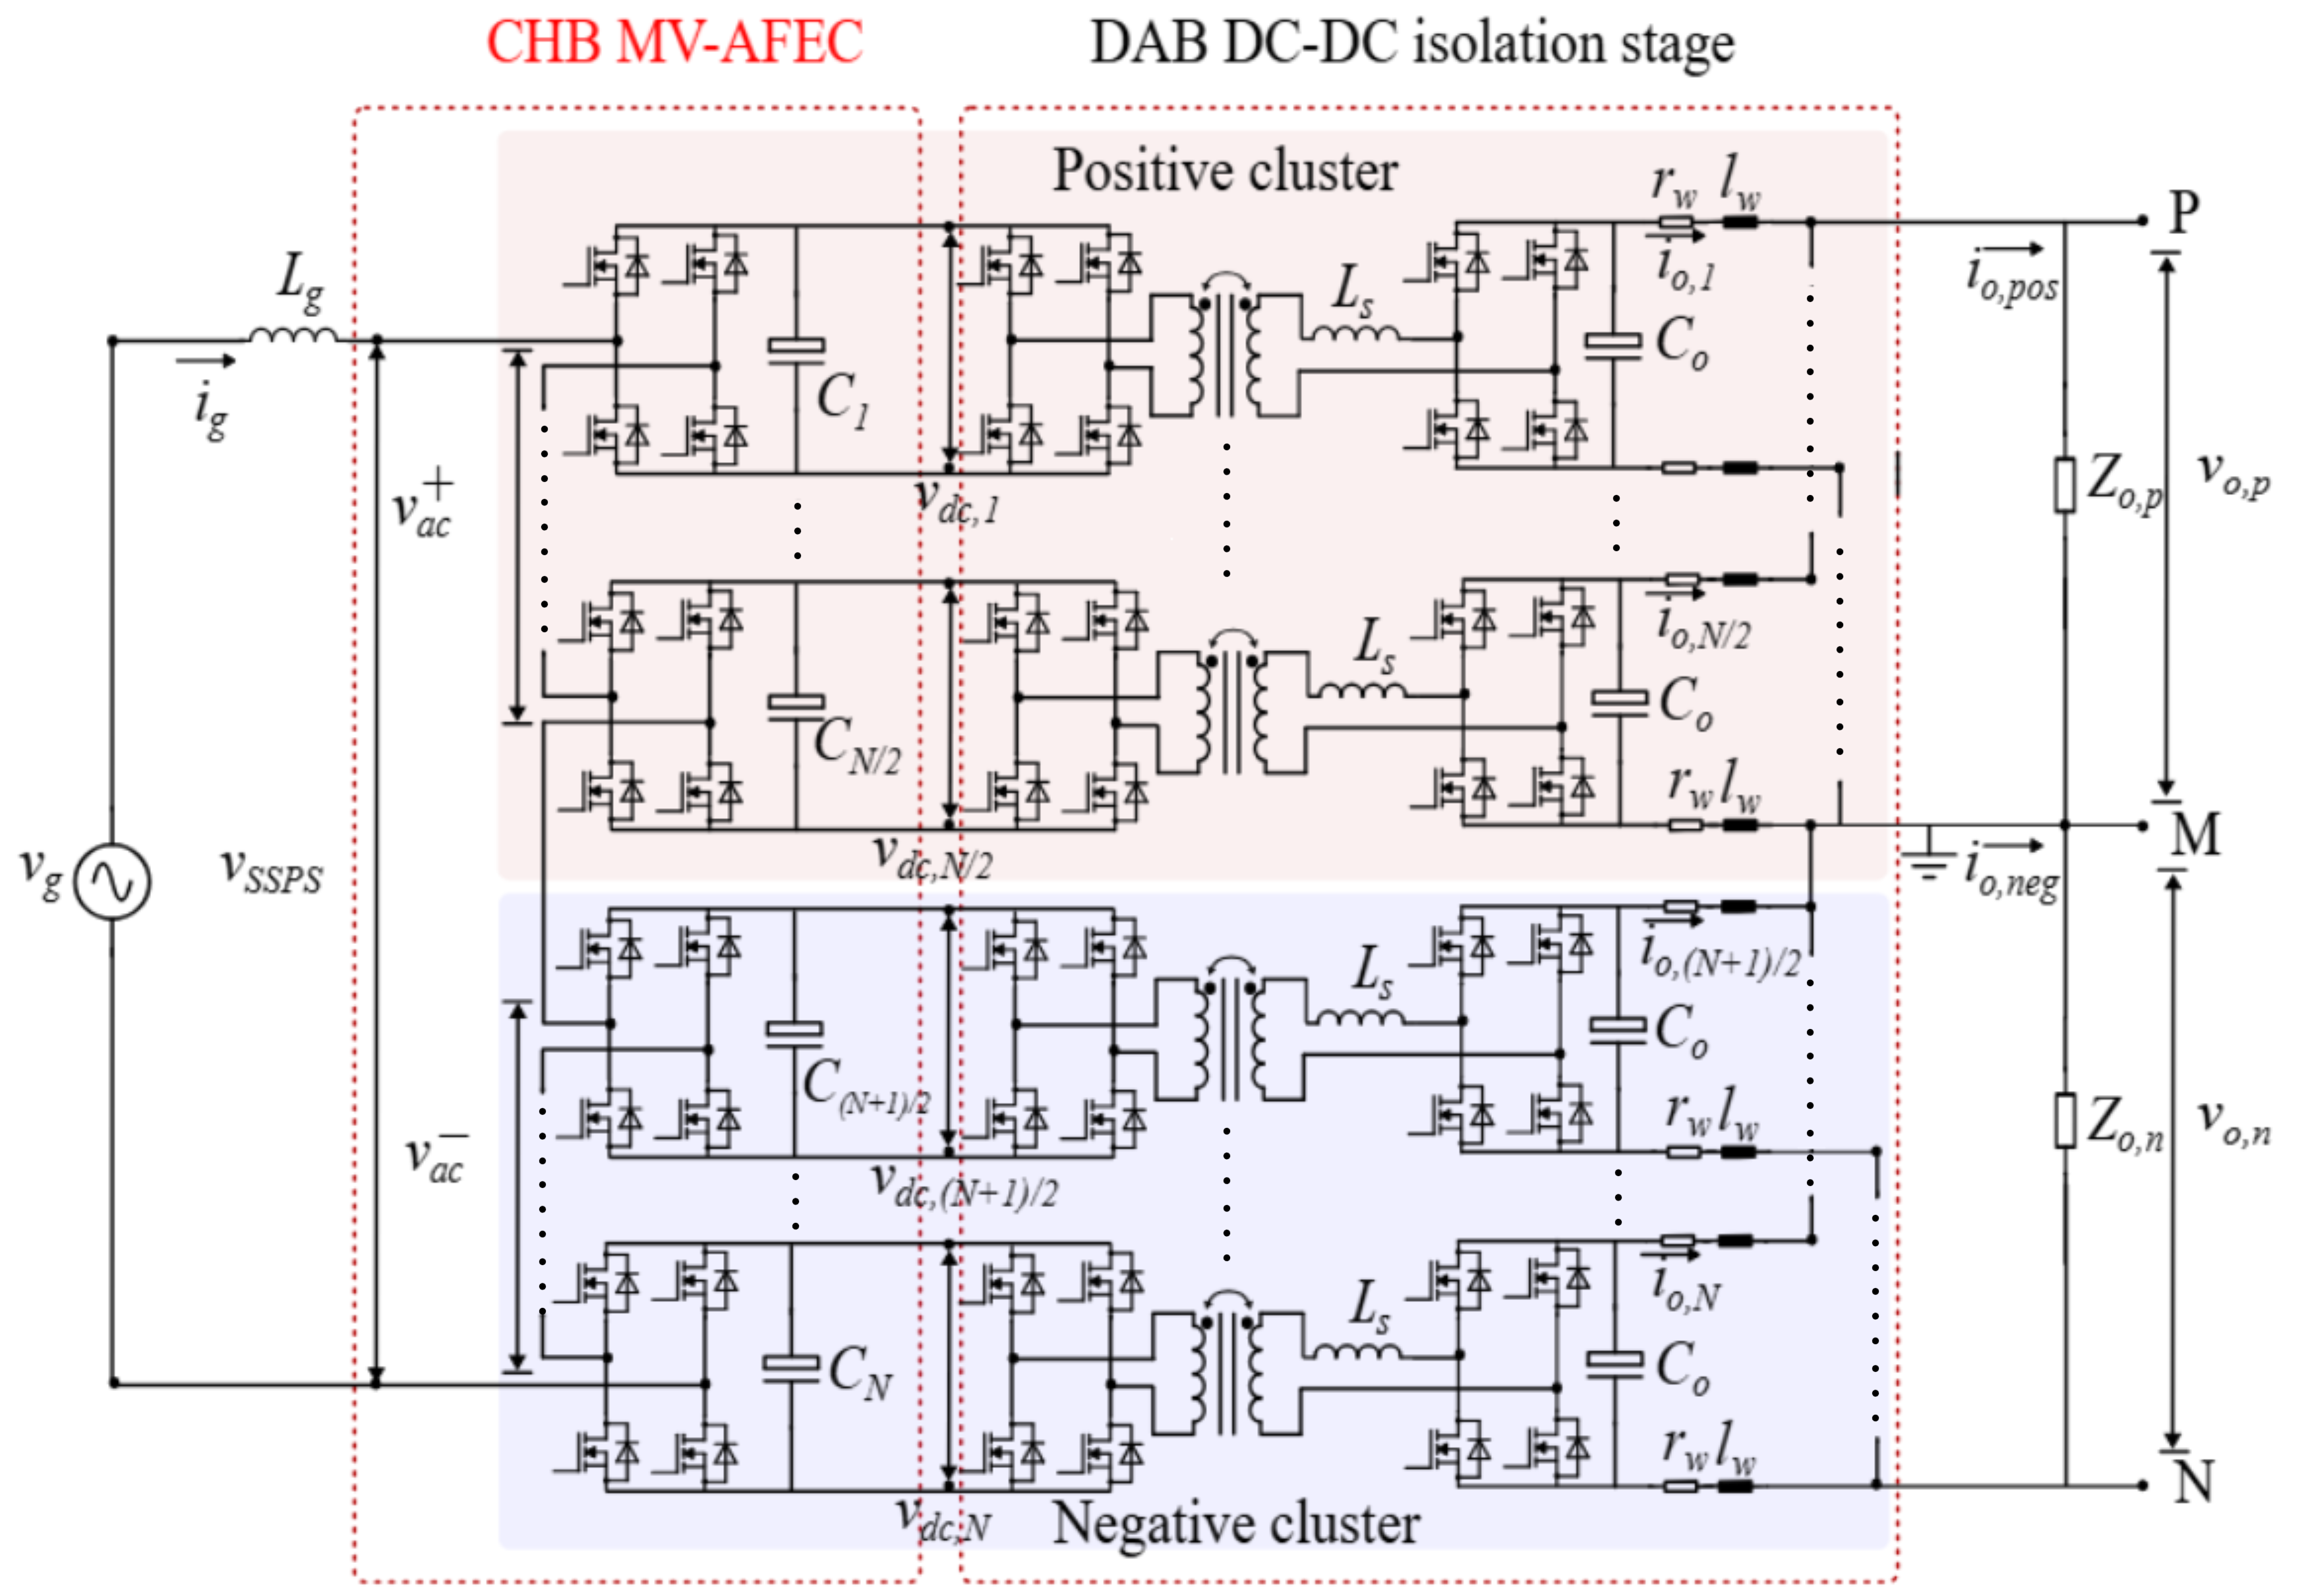
\includegraphics[width=\linewidth]{SSTS.png}
        \caption{Solid State Power Substation architecture.}
        \label{fig: SSPS schematic}
    \end{subfigure}

    \vspace{0.5em}

    \begin{subfigure}{0.7\textwidth}
        \centering
        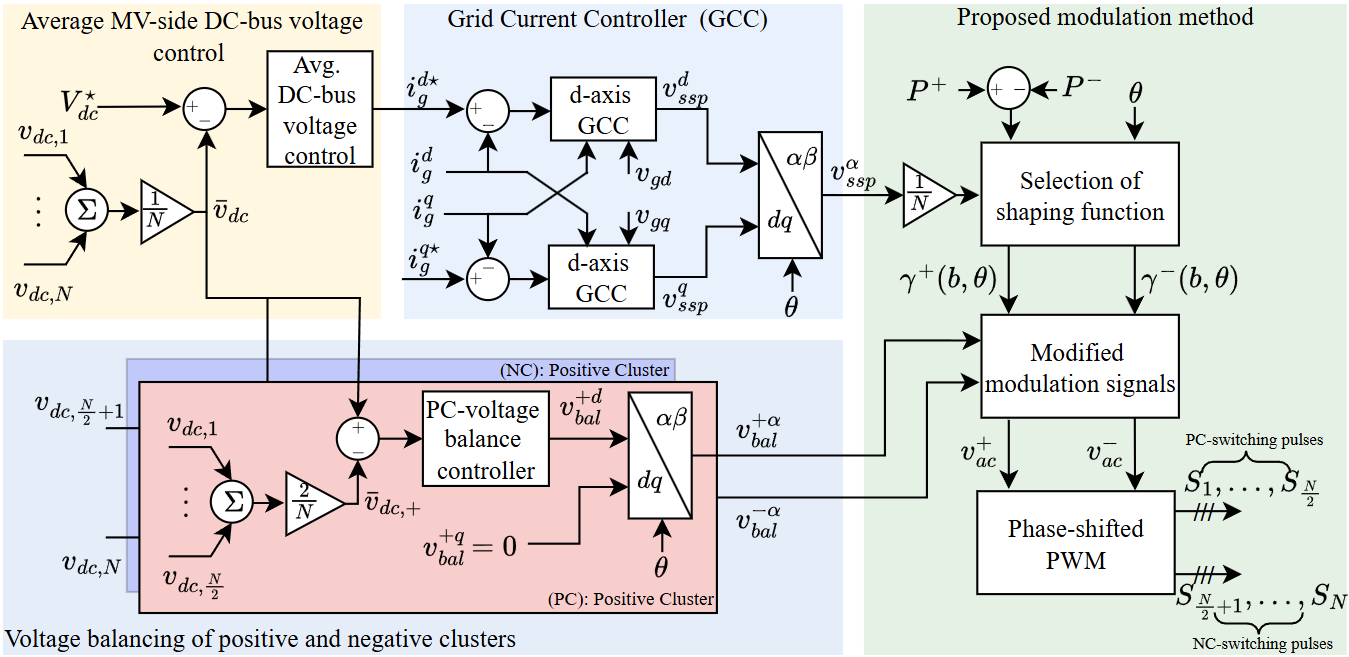
\includegraphics[width=\linewidth]{Control_BD_v1.png}
        \caption{CHB MV-AFEC control block diagram.}
        \label{fig: CHB_control_BD}
    \end{subfigure}

    \caption{System architecture and control structure of the proposed Solid-State Power Substation (SSPS).}
    \label{fig:SSPS_combined}
\end{figure*}

A well-known challenge in supplying bipolar DC loads is operation under a significant power imbalance between the positive and negative rails \cite{Bipolar_microgrid_overview}. In such conditions, the cascaded H-bridge (CHB) topology offers limited capability to redistribute power between clusters, since each CHB cell is coupled to an isolated DC--DC stage and direct energy exchange between clusters is not available. Consequently, several mitigation strategies involving additional hardware or modified DC--DC stages have been proposed in the literature \cite{Binbin_CFDAB}. In this work, control and modulation strategies for the CHB converter are developed to improve operation under unbalanced loading. The key contributions of this work are summarized as follows:

\begin{enumerate}
    \item Analysis of the SSPS operating range during unbalanced loading.
    \item A novel voltage shaping-function-based modulation technique that extends the SSPS operating range during unbalanced loading conditions.
\end{enumerate}

\section{Overview of the Proposed Control Approach}

The CHB control architecture consists of station-level, cluster-level, and cell-level control layers, as shown in \Cref{fig: CHB_control_BD}. At the station level, a synchronous reference-frame decoupled power controller regulates the power exchange with the grid while maintaining the average MV-side DC-bus voltage. At the cluster level, voltage-balancing controllers regulate the average DC-link voltage of the positive and negative clusters. The proposed modulation method is implemented at this level to increase the allowable range of unbalanced load operation. Finally, switching signals for individual CHB cells are generated using phase-shifted PWM.

\section{Cluster Power Sharing and Limitation of Linear Modulation}

The active power processed by the positive and negative clusters are given by \cref{eq:pos_power} and \cref{eq:neg_power}.

\begin{equation}
P^+ = M^+ V_{dc} I_g \cos\phi^+
\label{eq:pos_power}
\end{equation}

\begin{equation}
P^- = M^- V_{dc} I_g \cos\phi^-
\label{eq:neg_power}
\end{equation}

where $M^+$ and $M^-$ denote the modulation indices of the positive and negative clusters, $I_g$ is the RMS grid current, and $\phi^+$ and $\phi^-$ are the corresponding power-factor angles. The expressions for \(M^{+}\) and \(M^{-}\) as a function of the cluster power ratio \(a = P^{+}/P^{-}\) and designed station modulation index \(M_{des}\) are shown in \cref{eq:pos_mod} and \cref{eq:neg_mod}, respectively.

\begin{equation}
M^+ = \frac{2a}{1+a} M_{des}
\label{eq:pos_mod}
\end{equation}

\begin{equation}
M^- = \frac{2}{1+a} M_{des}
\label{eq:neg_mod}
\end{equation}

It can be shown that, under linear sinusoidal modulation, the requirement to avoid over-modulation limits the cluster power ratio to \(a \in [0.5,\,2]\) for \(M_{des}=0.75\)~\cite{Ko_clamped_pwm}. The next section presents the proposed approach to extend this range.

\section{Proposed Modulation Technique to Expand the Range of Unbalanced Power Operation}

To increase the allowable unbalanced operating range in linear sine modulation, the modulation waveform is reshaped to enhance the fundamental component while keeping $M^+$ and $M^-$ within unity. The proposed complementary shaping functions are

\begin{equation}
f(b,\theta) = M_{des}(\sin\theta)^{1/b}
\label{eq:f_eq}
\end{equation}

\begin{equation}
g(b,\theta) = 2M_{des}\sin\theta - f(b,\theta)
\label{eq:g_eq}
\end{equation}

where $b$ is a bulge factor~\cite{Mouli_bulge_factor} that controls the increase of the fundamental component in $f(b,\theta)$. The function $g(b,\theta)$ is defined such that $f(b,\theta)+g(b,\theta)$ results in a sinusoidal station-level modulation waveform. \Cref{fig:bulge_f_theta} and \cref{fig:bulge_g_theta} illustrate the shaping functions $f(b,\theta)$ and $g(b,\theta)$, respectively, for $b=1,2,3,$ and $100$, while \cref{fig:bulge_fg} shows the variation of the magnitudes of their fundamental components as a function of $b$.

Since $f(b,\theta)$ provides a larger fundamental component, it is applied to the cluster supplying the higher load, while the other cluster uses $g(b,\theta)$, as implemented in the modulation selection block in \Cref{fig: CHB_control_BD}. The resulting cluster modulation signals are

\begin{equation}
\gamma^+(b,\theta) =
\begin{cases}
f(b,\theta), & \text{if } P_o^+ \ge P_o^- \\
g(b,\theta), & \text{if } P_o^+ \le P_o^-
\end{cases}
\label{eq:f_pos_fun}
\end{equation}

\begin{equation}
\gamma^-(b,\theta) =
\begin{cases}
f(b,\theta), & \text{if } P_o^- \ge P_o^+ \\
g(b,\theta), & \text{if } P_o^- \le P_o^+
\end{cases}
\label{eq:f_neg_fun}
\end{equation}

The cluster voltage-balancing outputs (shown in \cref{fig: CHB_control_BD}) are then combined with the proposed modulation signals in \cref{eq:vac_plus_eq} and \cref{eq:vac_minus_eq} to generate the PWM references \(v^{+}_{ac}\) and \(v^{-}_{ac}\).

\begin{equation}
v_{ac}^{+} = v_{bal}^{+\alpha} + \gamma^{+}(b,\theta)
\label{eq:vac_plus_eq}
\end{equation}

\begin{equation}
v_{ac}^{-} = v_{bal}^{-\alpha} + \gamma^{-}(b,\theta)
\label{eq:vac_minus_eq}
\end{equation}

\begin{figure*}[t]
    \centering
    \begin{subfigure}[t]{0.32\textwidth}
        \centering
        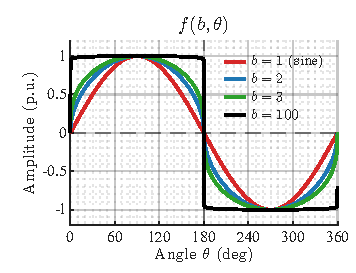
\includegraphics[width=\textwidth]{bulge_f_theta_v0.pdf}
        \caption{}
        \label{fig:bulge_f_theta}
    \end{subfigure}
    \hfil
    \begin{subfigure}[t]{0.32\textwidth}
        \centering
        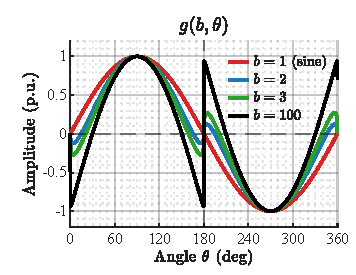
\includegraphics[width=\textwidth]{bulge_g_theta_v0.pdf}
        \caption{}
        \label{fig:bulge_g_theta}
    \end{subfigure}
    \hfil
    \begin{subfigure}[t]{0.32\textwidth}
        \centering
        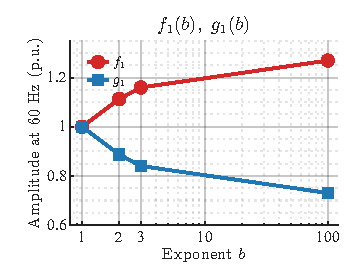
\includegraphics[width=\textwidth]{bulge_fg_60Hz_v0.pdf}
        \caption{}
        \label{fig:bulge_fg}
    \end{subfigure}
    \caption{Proposed modulation shaping functions: (a) $f(b,\theta)$, (b) $g(b,\theta)$, and (c) variation of per unit fundamental component of \(f_{1}(b,\theta)\) and \(g_{1}(b,\theta)\) with exponent \(b\).}
    \label{fig:proposed_modulation_functions}
\end{figure*}

The effectiveness of the proposed modulation method is evaluated using PLECS simulations of the SSPS described in \cref{sec: Intro} with an unbalanced load ratio $a=2$ applied at $t=0.1$\,s. In \Cref{fig:sim_sine_a}, linear sinusoidal modulation fails to maintain DC-link voltage regulation at this operating point, as $a=2$ corresponds to the theoretical operating boundary under this modulation technique. In contrast, the proposed modulation method with bulge factor $b=2$ achieves stable operation in \Cref{fig:sim_prop_b}. The effect of the bulge factor on the allowable unbalanced operating range is shown in \Cref{fig:sim_range_c}, where increasing $b$ extends the operating boundary.

\begin{figure*}[t]
    \centering
    \begin{subfigure}[t]{0.3\textwidth}
        \centering
        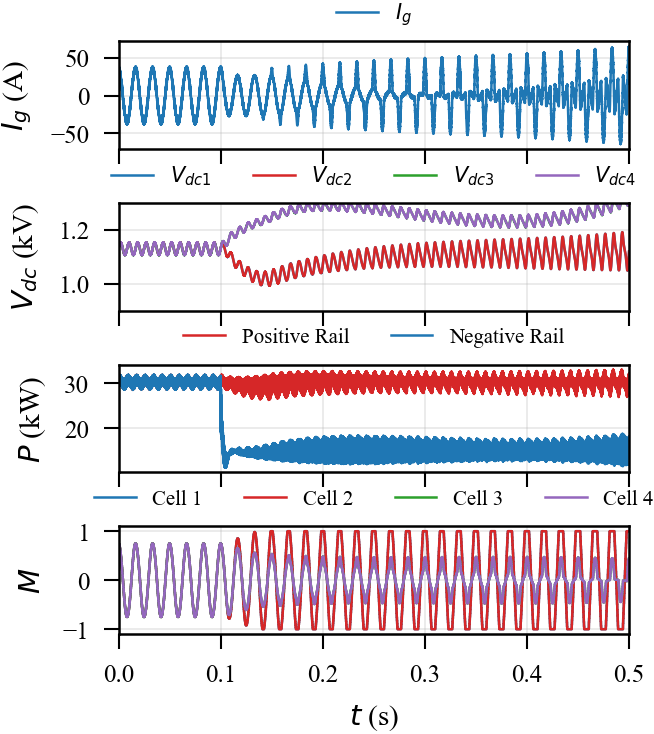
\includegraphics[width=\textwidth]{Fig1_Sine_Modulation_4x1.png}
        \caption{}
        \label{fig:sim_sine_a}
    \end{subfigure}
    \hfill
    \begin{subfigure}[t]{0.3\textwidth}
        \centering
        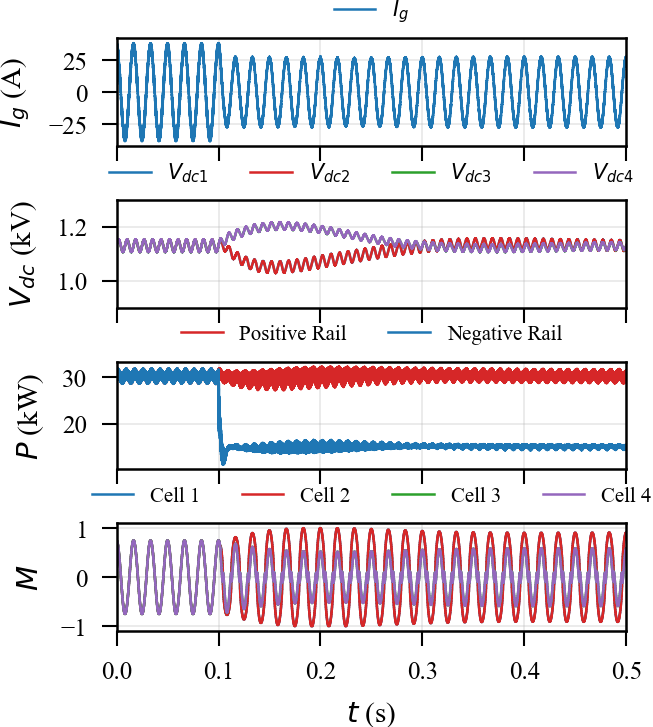
\includegraphics[width=\textwidth]{Fig2_Proposed_Modulation_4x1.png}
        \caption{}
        \label{fig:sim_prop_b}
    \end{subfigure}
    \hfill
    \begin{subfigure}[t]{0.3\textwidth}
        \centering
        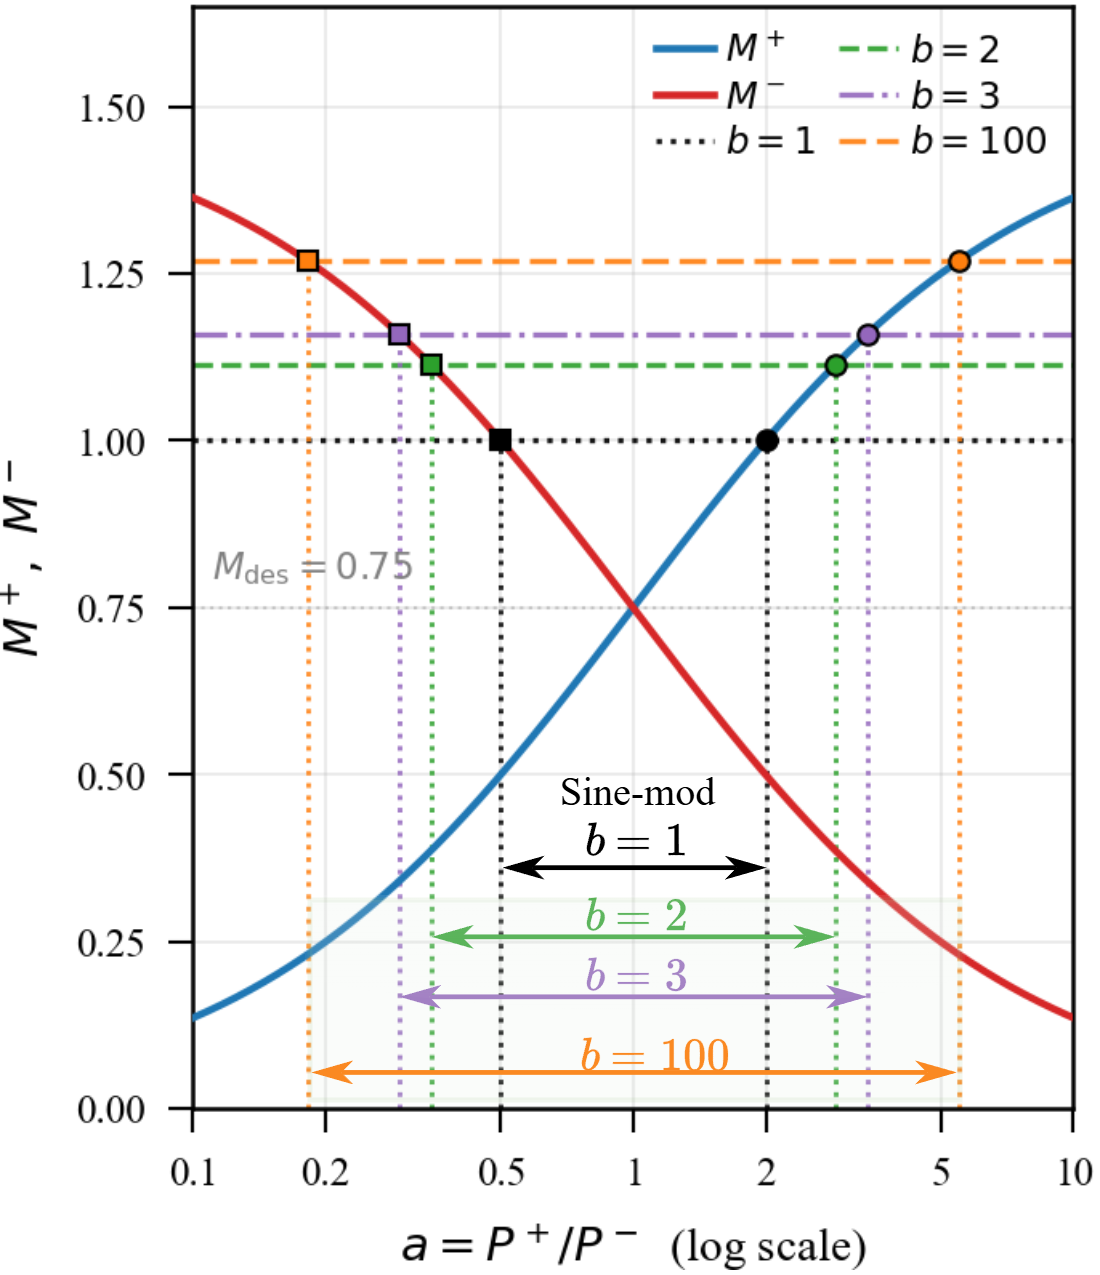
\includegraphics[width=\textwidth]{MI_curves_v0_ann.png}
        \caption{}
        \label{fig:sim_range_c}
    \end{subfigure}
    \caption{Simulation plots of SSPS operation when the negative rail load power decreases by 0.5 p.u. (a) Linear sine modulation technique; (b) Proposed modulation technique; (c) Limits of unbalanced operating regions.}
    \label{fig:simulation_results}
\end{figure*}

\section{Experimental Setup and Preliminary Validation}

To validate the operation under unbalanced loading, a low-voltage experimental prototype shown in \cref{fig:exp_setup} is built, and the system parameters are shown in \Cref{tab:lv_ssps_sys_param}. A preliminary scope capture of the SSPS during unbalanced loading using the proposed modulation is shown in \cref{fig:exp_result}. An unbalanced load of $a=2.33$ is applied to the positive and negative clusters. The CHB is modulated using the proposed method with a bulge factor of 2. The analysis presented in \cref{fig:sim_range_c} suggests that a bulge factor of 2 is appropriate for the applied load imbalance. In the full paper, the operation under varying bulge factors and its implications on the allowed power imbalance will be experimentally verified.

\begin{table}[htbp]
\caption{Low Voltage Prototype SSPS System Parameters}
\centering
\footnotesize
\begin{tabular}{lc}
\toprule
Parameter & Value \\
\midrule
Interconnection Voltage & $210\,\mathrm{V}_{l\text{-}n,\mathrm{rms}},~60\,\mathrm{Hz}$ \\
Rated Power & $1\,\mathrm{kVA}$ \\
Number of cells & 2 \\
CHB DC-link voltage ($V_{dc}$) & $200\,\mathrm{V}$ \\
Station output voltage ($V_o$) & $\pm 200\,\mathrm{V}$ \\
CHB modulation index & 0.75 \\
\bottomrule
\end{tabular}
\label{tab:lv_ssps_sys_param}
\end{table}

\begin{figure}[htbp]
    \centering
    \begin{subfigure}[t]{0.45\columnwidth}
        \centering
        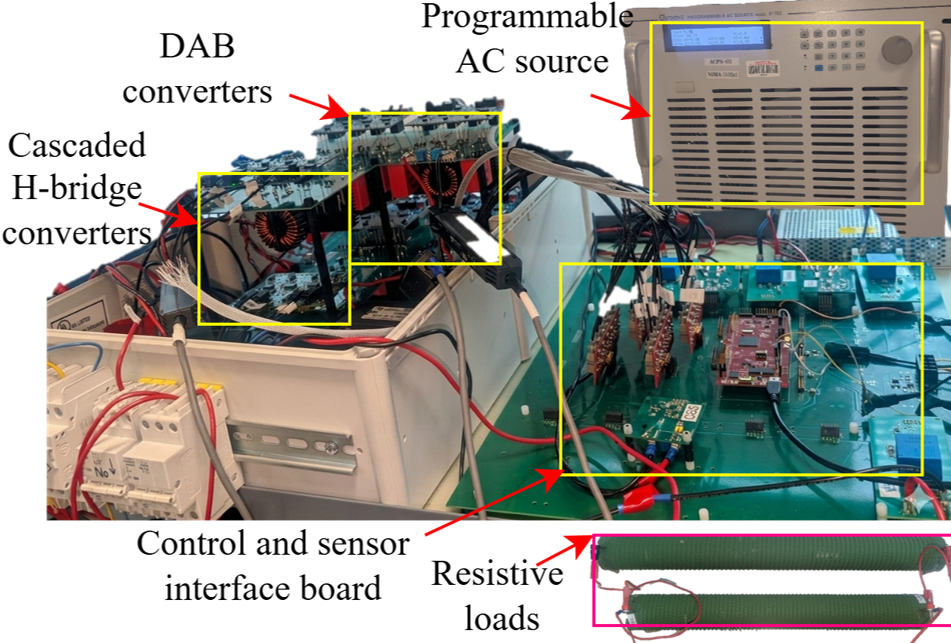
\includegraphics[width=\textwidth]{Experimental_setup.png}
        \caption{}
        \label{fig:exp_setup}
    \end{subfigure}
    \hfill
    \begin{subfigure}[t]{0.50\columnwidth}
        \centering
        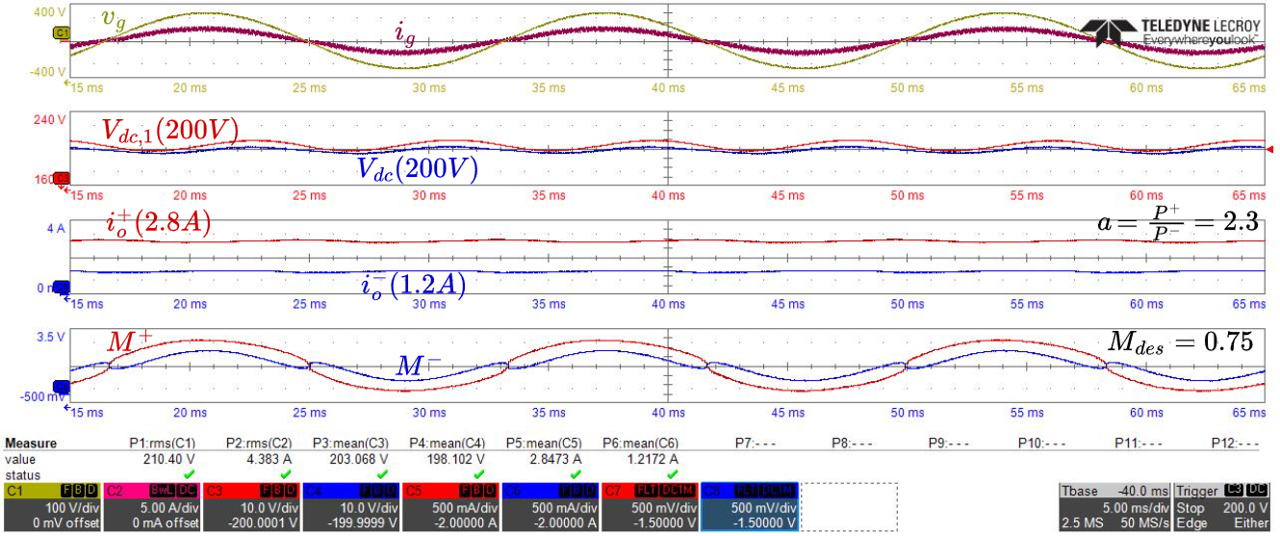
\includegraphics[width=\textwidth]{Exp_result.png}
        \caption{}
        \label{fig:exp_result}
    \end{subfigure}
    \caption{(a) A photograph of the experimental low-voltage prototype; (b) Preliminary scope capture of the 2-cell CHB operation with proposed modulation method at an unbalanced load ratio, \(a = 2.33\).}
    \label{fig:experimental}
\end{figure}

\section{Conclusion}

Conventional linear sinusoidal modulation is limited by the amplitude of the modulating signal, restricting the allowable unbalanced operating range. This paper proposes a shaping-function-based modulation strategy to extend the operating range of a CHB-SST supplying unbalanced bipolar DC loads. Without affecting the station voltage, the proposed method increases the fundamental voltage component of the higher-load cluster while proportionally reducing that of the lower-load cluster. The analysis is validated through simulation and experimental results, demonstrating an extended unbalanced operating range compared to conventional sinusoidal modulation. The full paper will further investigate the impact of injected cluster-level harmonic voltages on the DC side across various power factors, present a systematic method for selecting the bulge factor, including associated design considerations, and provide detailed experimental validation.

\bibliographystyle{IEEEtran}
\bibliography{IEEEabrv,Bibliography}

\end{document}
